%%%%%%%%%%%%%%%%%%%%%%%%%%%%%%%%%%%%%%%%%
% Simple Sectioned Essay Template
% LaTeX Template
%
% This template has been downloaded from:
% http://www.latextemplates.com
%
% Note:
% The \lipsum[#] commands throughout this template generate dummy text
% to fill the template out. These commands should all be removed when 
% writing essay content.
%
%%%%%%%%%%%%%%%%%%%%%%%%%%%%%%%%%%%%%%%%%

%----------------------------------------------------------------------------------------
%	PACKAGES AND OTHER DOCUMENT CONFIGURATIONS
%----------------------------------------------------------------------------------------

%\documentclass[12pt]{article} % Default font size is 12pt, it can be changed here

%\usepackage{geometry} % Required to change the page size to A4
%\geometry{letterpaper} % Set the page size to be A4 as opposed to the default US Letter

%\usepackage{graphicx} % Required for including pictures

%\usepackage{listings} %Para comandos bash Linux

%\usepackage{float} % Allows putting an [H] in \begin{figure} to specify the exact location of the figure
%\usepackage{wrapfig} % Allows in-line images such as the example fish picture

%\usepackage{color} %textos de colores

%\usepackage[spanish]{babel}

%\usepackage[utf8]{inputenc} %Uso de acentos directamente

%\usepackage{hyperref}

%\linespread{1.2} % Line spacing

%\setlength\parindent{0pt} % Uncomment to remove all indentation from paragraphs

%\graphicspath{{Pictures/}} % Specifies the directory where pictures are stored

%\begin{document}

%----------------------------------------------------------------------------------------
%	TITLE PAGE
%----------------------------------------------------------------------------------------

%\begin{titlepage}

%\newcommand{\HRule}{\rule{\linewidth}{0.5mm}} % Defines a new command for the horizontal lines, change thickness here

%\center % Center everything on the page

%\textsc{\LARGE Universidad Autónoma de Yucatán}\\[1.5cm] % Name of your university/college
%\textsc{\Large Facultad de Matemáticas}\\[0.5cm] % Major heading such as course name
%\textsc{\large Anexo de tesis de Alex Antonio Turriza Suárez}\\[0.5cm] % Minor heading such as course title

%\HRule \\[0.4cm]
%{ \huge \bfseries Configuración de los Dispositivos GPS Ublox C94-M8P para su uso en RTKLIB}\\[0.4cm] % Title of your document
%\HRule \\[1.5cm]
%\begin{minipage}{0.5\textwidth}
%\begin{flushleft} \large
%\emph{Autor:}\\
%Alex Antonio \textsc{Turriza Suárez} % Your name
%\end{flushleft}
%\end{minipage}
%~
%\begin{minipage}{0.4\textwidth}
%\begin{flushright} \large
%\emph{Asesores:} \\
%Dr. Arturo \textsc{Espinosa Romero} \\
%\ \ \\
%Dr. Anabel \textsc{Martín González}
%\end{flushright}
%\end{minipage}\\[4cm]

%{\large \today}\\[3cm] % Date, change the \today to a set date if you want to be precise

%\includegraphics{Logo}\\[1cm] % Include a department/university logo - this will require the graphicx package

%\vfill % Fill the rest of the page with whitespace

%\end{titlepage}

%----------------------------------------------------------------------------------------
%	TABLE OF CONTENTS
%----------------------------------------------------------------------------------------

%\tableofcontents % Include a table of contents

%\newpage % Begins the essay on a new page instead of on the same page as the table of contents 

%----------------------------------------------------------------------------------------
%	INTRODUCTION
%----------------------------------------------------------------------------------------
\chapter{Configuración del GPS Ublox C94-M8P para su uso en RTKLIB}\label{Anx:ublox}
\section{Introducción}
Para el uso del sistema GPS en modo cinemático, es necesario contar con dos dispositivos en dos roles diferentes: uno que brinde información de posicionamiento en modo estático en un marco de referencia terrestre, llamado \textit{Estación base}, con coordenadas conocidas; y otro, que brinde información de posicionamiento de un equipo en movimiento, llamado \textit{Rover} o \textit{Estación móvil}.\\

Configuradas de esta manera, RTKLIB puede procesar los datos de ambas para ofrecer una información depurada de posicionamiento del Rover.  

%------------------------------------------------

\section{Descripción de los componentes}\label{sec:Desc}
El kit de GPS Ublox C94-M8P proporciona:

\begin{itemize}
\item Un par de equipos GPS.
\item Un par de antenas UHF.
\item Un par de antenas GNSS.
\item Un par de cables de conexión USB-microUSB. 
\end{itemize}

%------------------------------------------------

\subsection{Preparando el dispositivo} % Sub-section

Para obtener un dispositivo funcional, hay que tomar un GPS y conectarle una antena UHF al conector marcado para dicha funcionalidad, una antena GNSS al conector indicado, y finalmente, colocarle el cable USB-microUSB al conector microUSB. De igual manera, se realiza para el otro GPS.

\section{Instalación en PC}\label{sec:InstPC}
En una PC con Windows, realizar los pasos descritos en las siguientes subsecciones.

\subsection{Descargas e Instalaciones}

\subsubsection{Software}

El primer paso es descargar el sofware de Ublox, de la liga: \href{https://www.u-blox.com/en/product/u-center-windows}{https://www.u-blox.com/en/product/u-center-windows}. Se abrirá una página web tal y como muestra la figura~\ref{fig:UbloxWeb}.

\begin{figure}[H] % Example image
\center{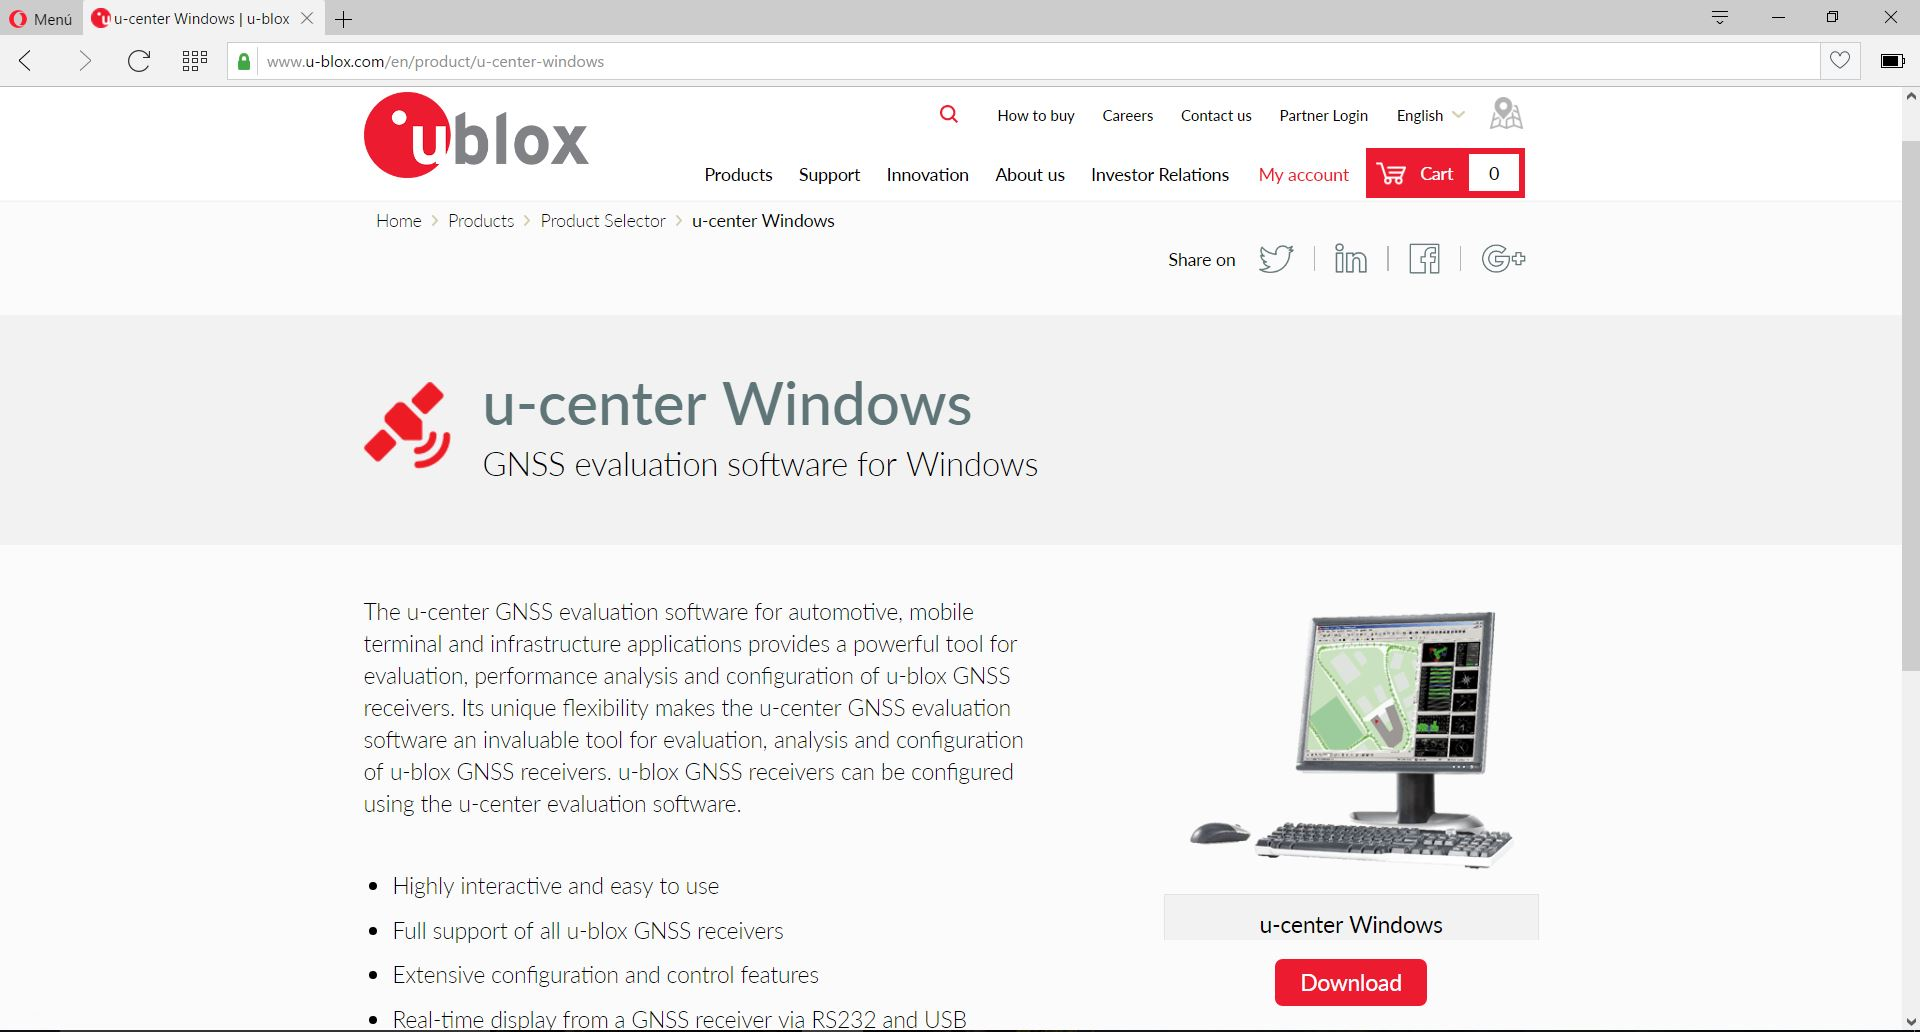
\includegraphics[width=0.9\linewidth]{Figures/Ublox/web}}
\caption{Página web de Ublox.}
\label{fig:UbloxWeb}
\end{figure}

Dar clic al botón de "Descargar", se obtendrá un archivo con extensión .exe. Instalar siguiendo los pasos indicados por el asistente y esperar a que termine la copia de archivos e instalación de drivers.\\

\newpage

Al final, buscar el lanzador de la aplicación de U-Center en el menú Inicio o bien en el escritorio, con un ícono como muestra la figura~\ref{fig:iconoUCenter}.

\begin{figure}[H] % Example image
\center{
\includegraphics[width=0.45\linewidth]{Figures/Ublox/icono}}
\caption{Software U-Center.}
\label{fig:iconoUCenter}
\end{figure}

\subsubsection{Drivers}

Para la correcta interpretación de los datos en formato RAW propietario enviados por el GPS, es necesario que los drivers sean instalados en Windows.\\

Tomar el cable USB-microUSB y conectar a un puerto USB de la computadora con Windows. Esperar a que detecte y se debe mostrar una ventana de instalación de drivers automático, como muestra la figura~\ref{fig:asisdriv}.

\begin{figure}[H] % Example image
\center{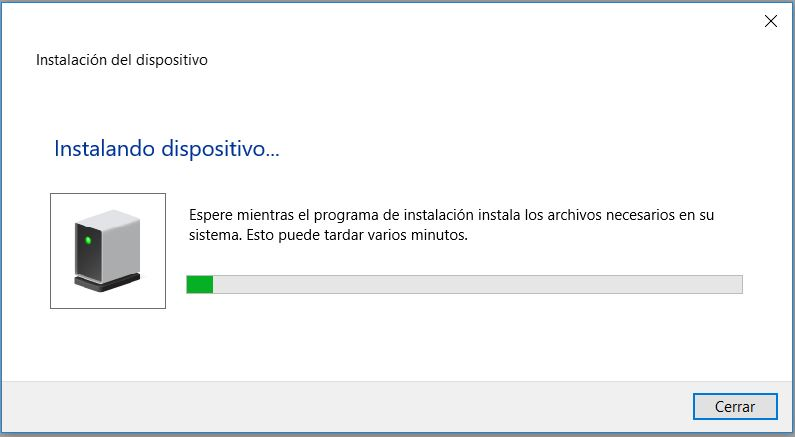
\includegraphics[width=0.9\linewidth]{Figures/Ublox/asisdrivers}}
\caption{Asistente de instalación de drivers.}
\label{fig:asisdriv}
\end{figure}

Al finalizar esa instalación, cerrar la ventana y verificar que haya sido correcta de la siguiente manera: Dar clic derecho al menú de inicio, y escoger \textbf{Administrador de Dispositivos}, tal y como muestra la figura~\ref{fig:startlist}.

\begin{figure}[H] % Example image
\center{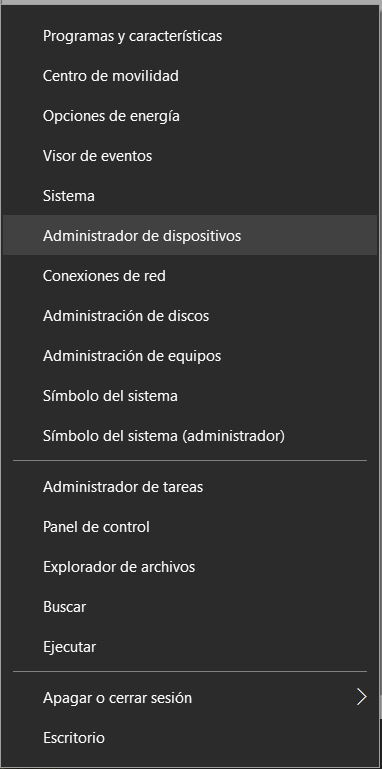
\includegraphics[width=0.53\linewidth]{Figures/Ublox/rightClic}}
\caption{Lista desplegable del menú Inicio.}
\label{fig:startlist}
\end{figure}

En la ventana que se abre, en la lista, desplegar \textit{Puertos (COM y LPT)} y verificar que se encuentra sublistado dentro de dicha categoría \textbf{u-blox Virtual COM Port (COMX)}, como muestra la figura~\ref{fig:admdisp}.

\begin{figure}[H] % Example image
\center{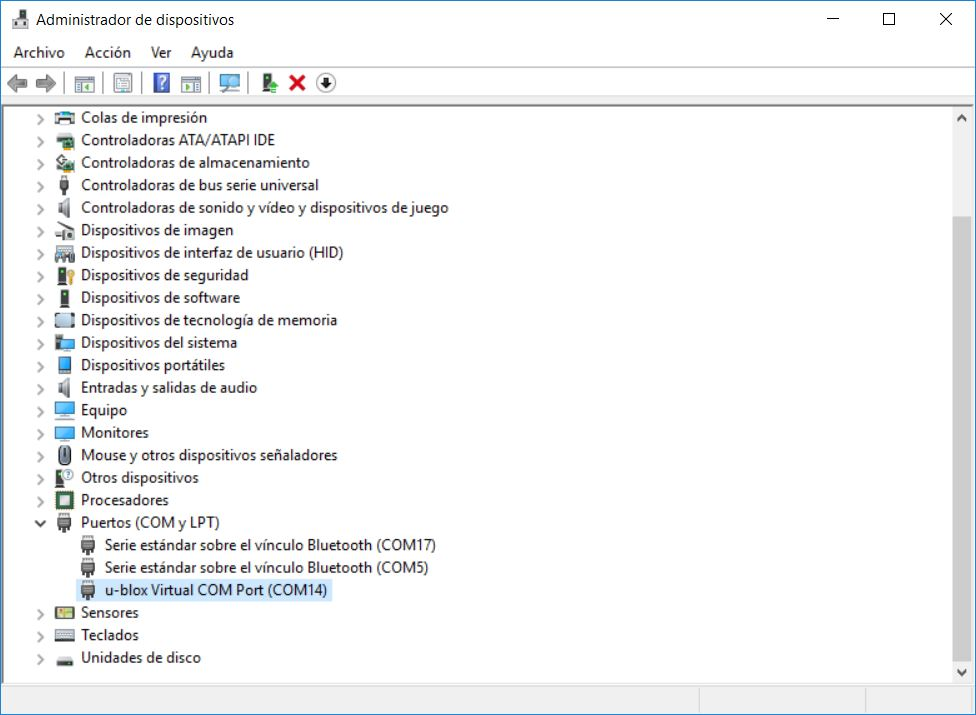
\includegraphics[width=0.89\linewidth]{Figures/Ublox/admdisp}}
\caption{Ventana principal del administrador de dispositivos.}
\label{fig:admdisp}
\end{figure}

\section{Configurando los GPS}\label{sec:Config}

\subsection{Configurar la estación base}\label{SubChap:ConfBase}

Abrir el software U-Center y conectar el GPS que será designado a ser de la estación base. Con el GPS correctamente conectado, se mostrará una imagen como la siguiente figura~\ref{fig:mainWind} en la ventana principal del programa.

\begin{figure}[H] % Example image
\center{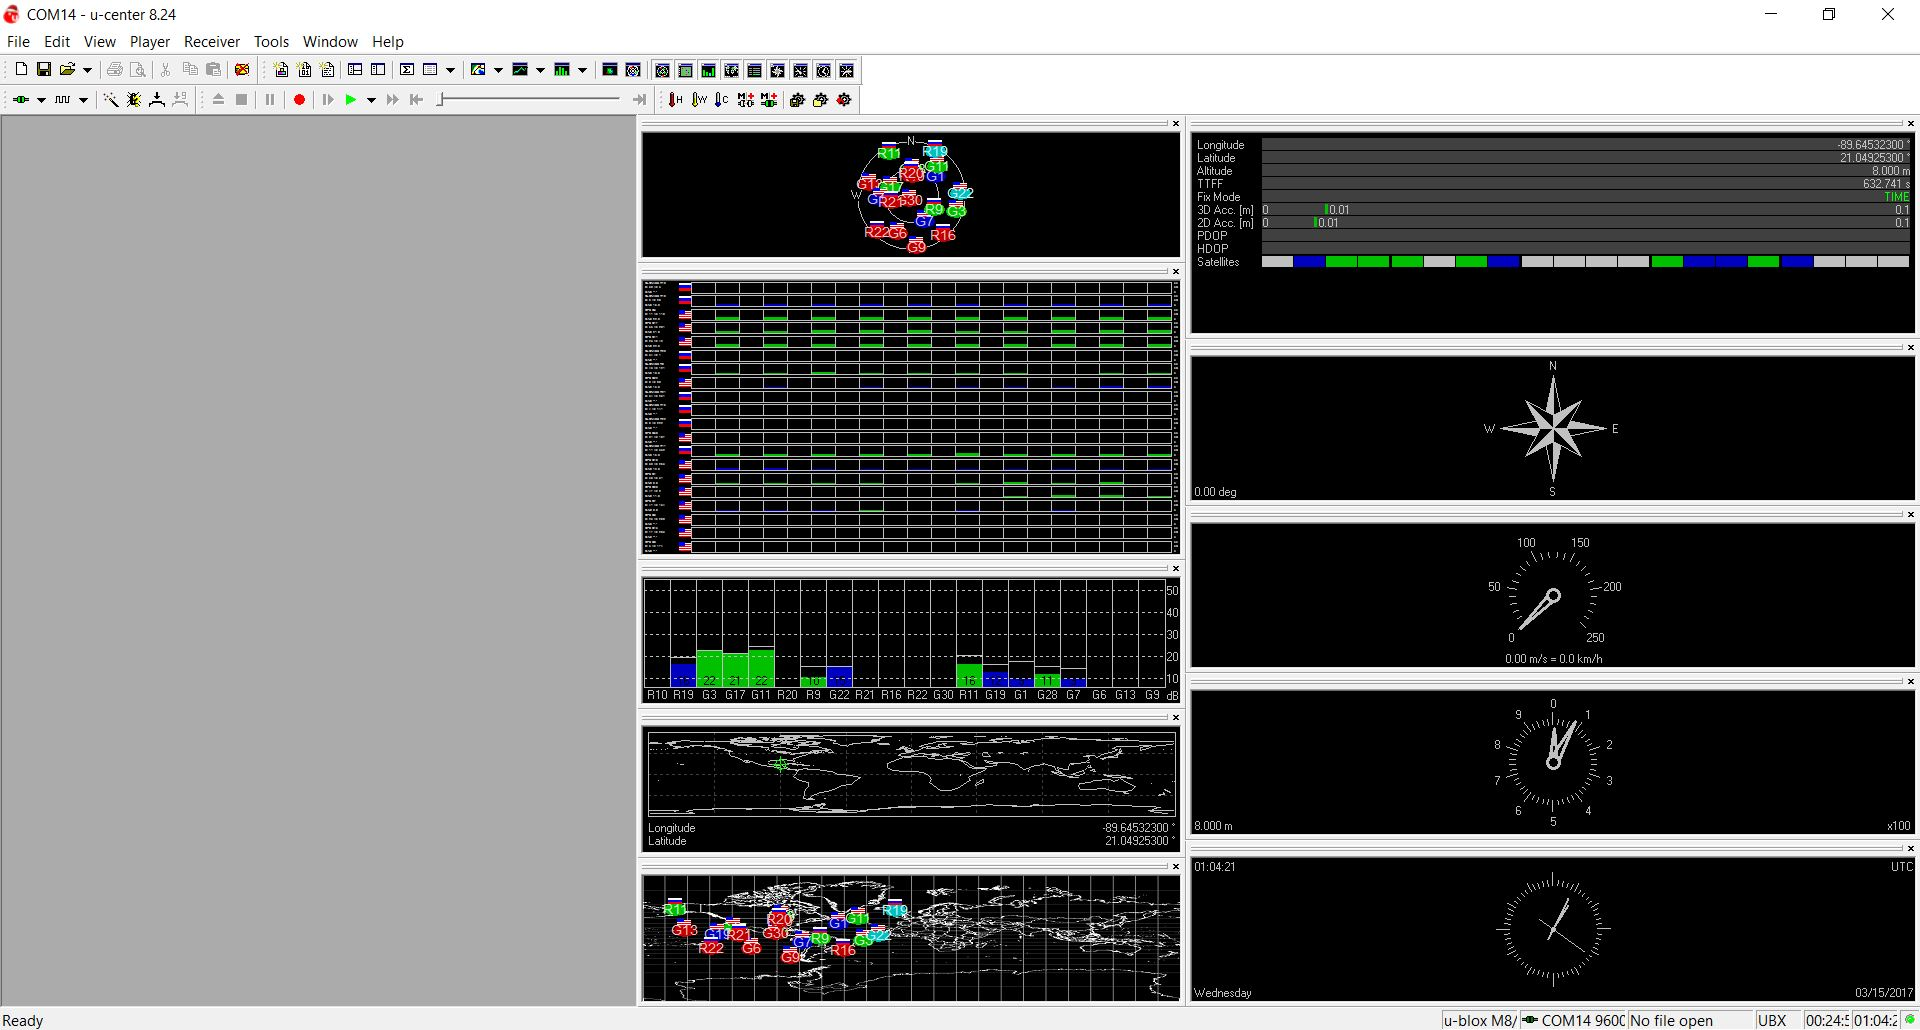
\includegraphics[width=0.95\linewidth]{Figures/Ublox/mainWind}}
\caption{Ventana principal de U-Center.}
\label{fig:mainWind}
\end{figure}

Del lado derecho de la ventana se despliega información diversa acerca de las observaciones actuales del GPS. En la parte inferior, en la barra de estado, se muestra info acerca del status actual del dispositivo (el tipo de mensaje enviado por el puerto USB, la tasa de baudios, el puerto al que está conectado a la PC, la hora del sistema satelital, entre otros.

Seleccionar la opción \textit{Messages View} a través del menú \textit{View}: \textbf{View $\rightarrow$ Messages View}, como muestra la figura \ref{fig:viewMView}. 

\begin{figure}[H] % Example image
\center{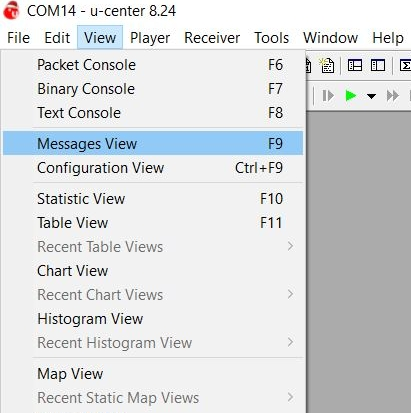
\includegraphics[width=0.75\linewidth]{Figures/Ublox/viewMView}}
\caption{Seleccionar la opción "Messages View" del menú "View".}
\label{fig:viewMView}
\end{figure}

Se abrirá una ventana en el área izquierda del programa U-Center, como la de la figura~\ref{fig:Messages}.

\begin{figure}[H] % Example image
\center{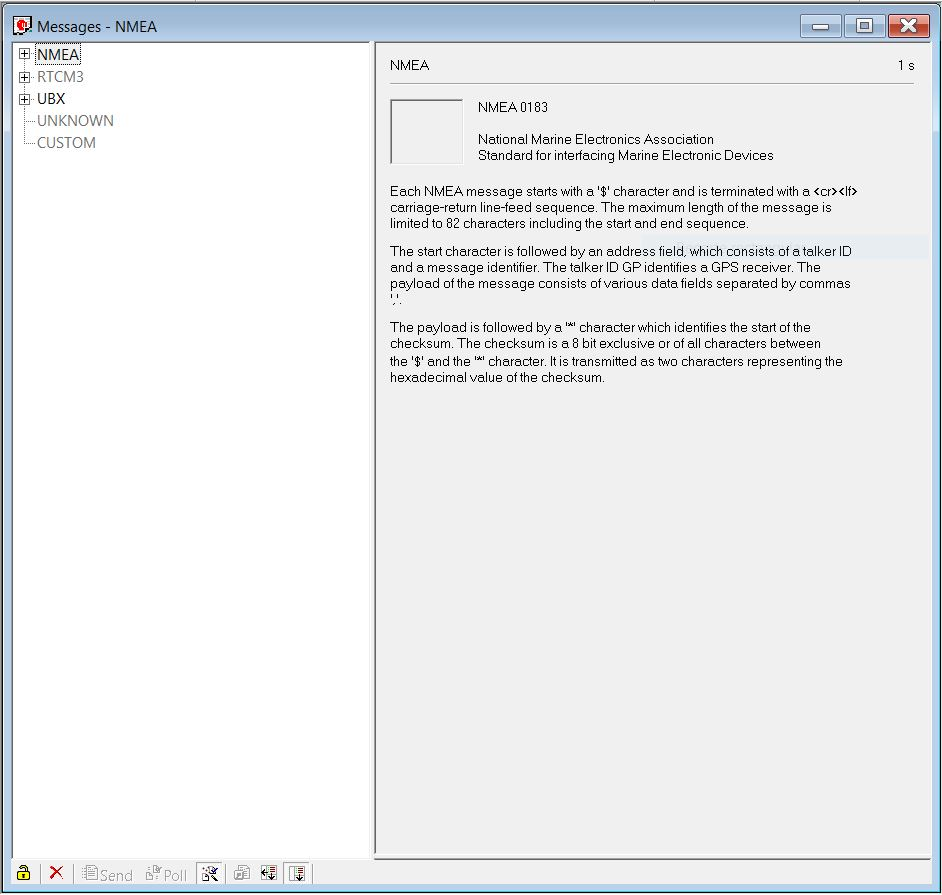
\includegraphics[width=0.8\linewidth]{Figures/Ublox/messages}}
\caption{Ventana de la opción "Messages".}
\label{fig:Messages}
\end{figure}

Dar clic derecho a \textbf{NMEA}, de la lista de la parte izquierda, y seleccionar \textit{Deshabilitar} del menú contextual. Ahora dar clic derecho a \textbf{UBX} y seleccionar \textit{Habilitar}.\\

En la lista de la izquierda, seguir la ruta: \textbf{UBX - CFG (Config) - TMODE3}. Saldrán unos cuadros de texto como muestra la figura~\ref{fig:TMode3Base}.

\begin{figure}[H] % Example image
\center{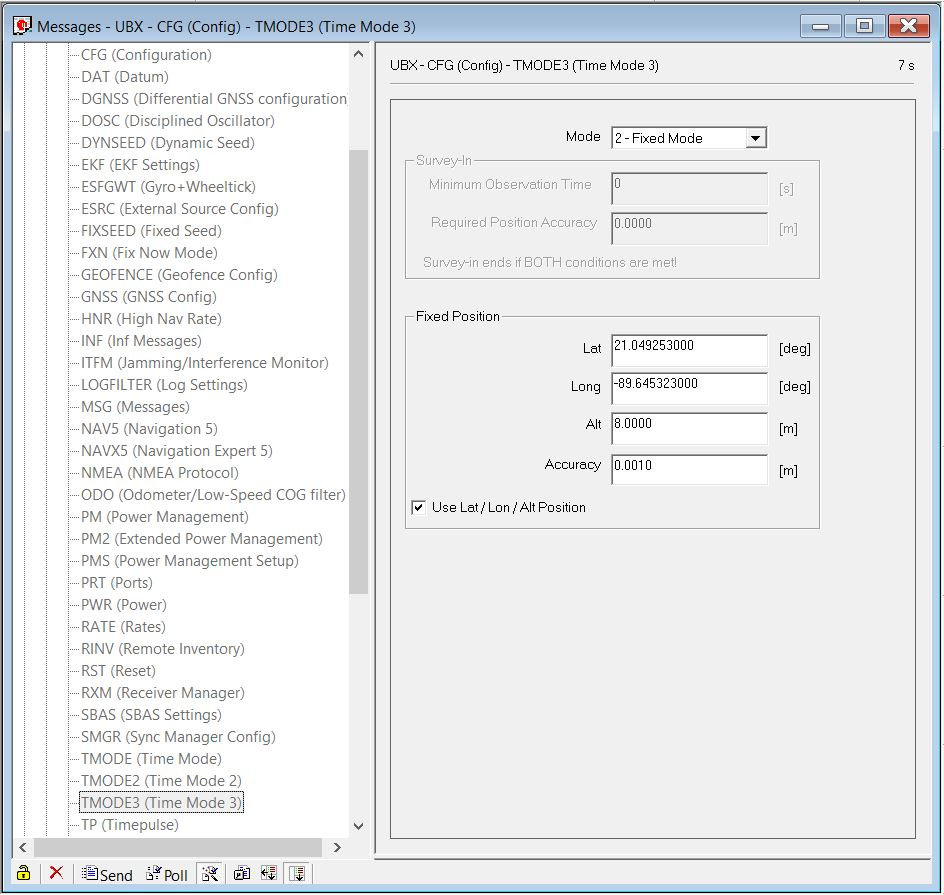
\includegraphics[width=0.75\linewidth]{Figures/Ublox/Captura9_Base}}
\caption{Opciones de la ventana "TMODE3".}
\label{fig:TMode3Base}
\end{figure}

Ahí, se introducirán los datos de localización de la estación base. Tal y como indica la figura \ref{fig:TMode3Base}, se ingresarán los siguientes datos a los cuadros de texto:

\begin{itemize}
\item \textbf{Mode}: \textit{2 - Fixed Mode}, para colocar coordenadas fijas de la estación base a utilizar.

\item Marcar \textit{Use Lat/Lon/Alt Position} en la parte inferior de la ventana.

\item \textbf{Lat:} Ingresar la latitud en grados.

\item \textbf{Long:} Ingresar la longitud en grados.

\item \textbf{Alt:} Ingresar la altura en metros sobre el nivel del mar.

\item \textbf{Accuracy:} Ingresar un factor de precisión en metros. Se recomienda utilizar 0.0010.
\end{itemize}

Finalmente, en la barra de herramientas situada en la barra inferior de la ventana, dar clic al botón \textbf{Send}, como el que muestra la figura~\ref{fig:SendButton}. 

\begin{figure}[H] % Example image
\center{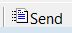
\includegraphics[width=0.3\linewidth]{Figures/Ublox/CapturaA}}
\caption{Botón "Send".}
\label{fig:SendButton}
\end{figure}

A continuación, en la lista de la izquierda, seguir la ruta: \textbf{UBX - CFG (Config) - PRT (Ports)}. \\

Aparecerá una ventana como la de la figura

\begin{figure}[H] % Example image
\center{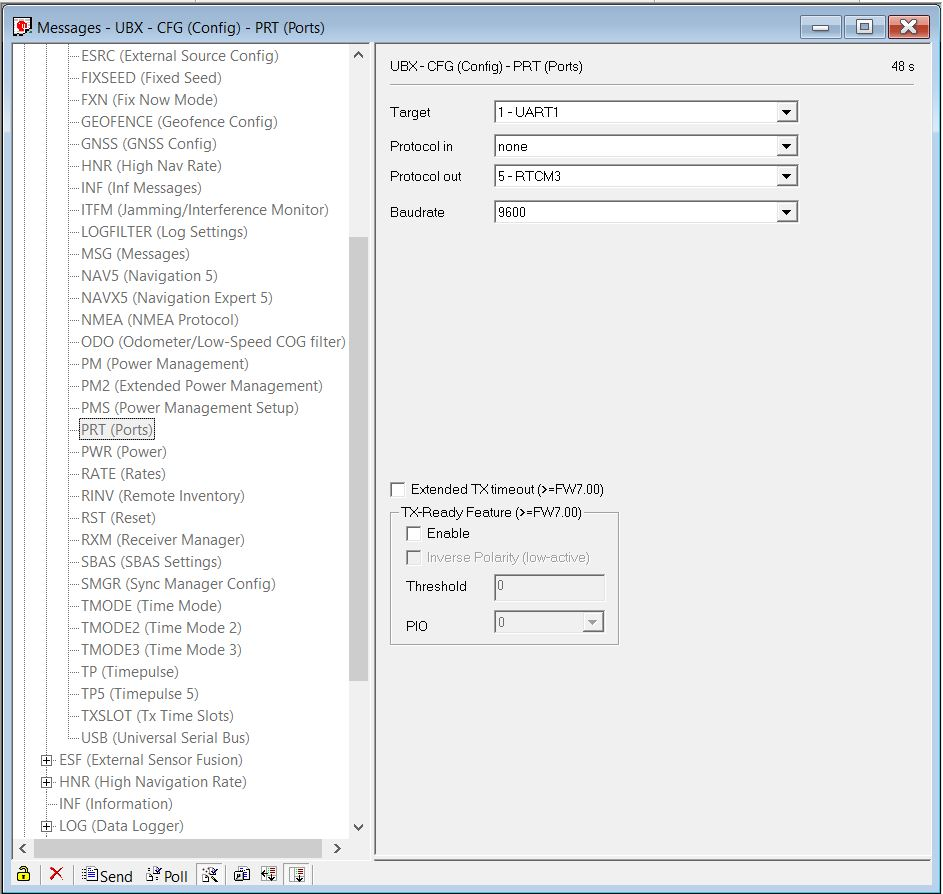
\includegraphics[width=0.6\linewidth]{Figures/Ublox/CapturaB_Base}}
\caption{Configuración de mensajes enviados inalámbricamente.}
\label{fig:PRT_Base}
\end{figure}

Aquí se ingresarán los datos a enviar mediante transmisión inalámbrica a través del puerto UART1. Se seleccionarán los siguientes parámetros:

\begin{itemize}
\item \textbf{Target}: \textit{1 - UART1}
\item \textbf{Protocol in}: \textit{none}
\item \textbf{Protocol out}: \textit{5-RTCM3}
\item \textbf{Baudrate}: \textit{9600}
\end{itemize}

Deshabilitar en caso de estar marcado \textit{Extended TX timeout(>=FW7.00)}.\\

Dar clic al botón \textbf{Send} de la barra de herramientas inferior.\\

A continuación, en la lista de la izquierda, seguir la ruta: \textbf{UBX - CFG (Config) - MSG (Messages)}. \\

Se muestra una ventana como la de la figura~\ref{fig:Mes_Base}. 

\begin{figure}[H] % Example image
\center{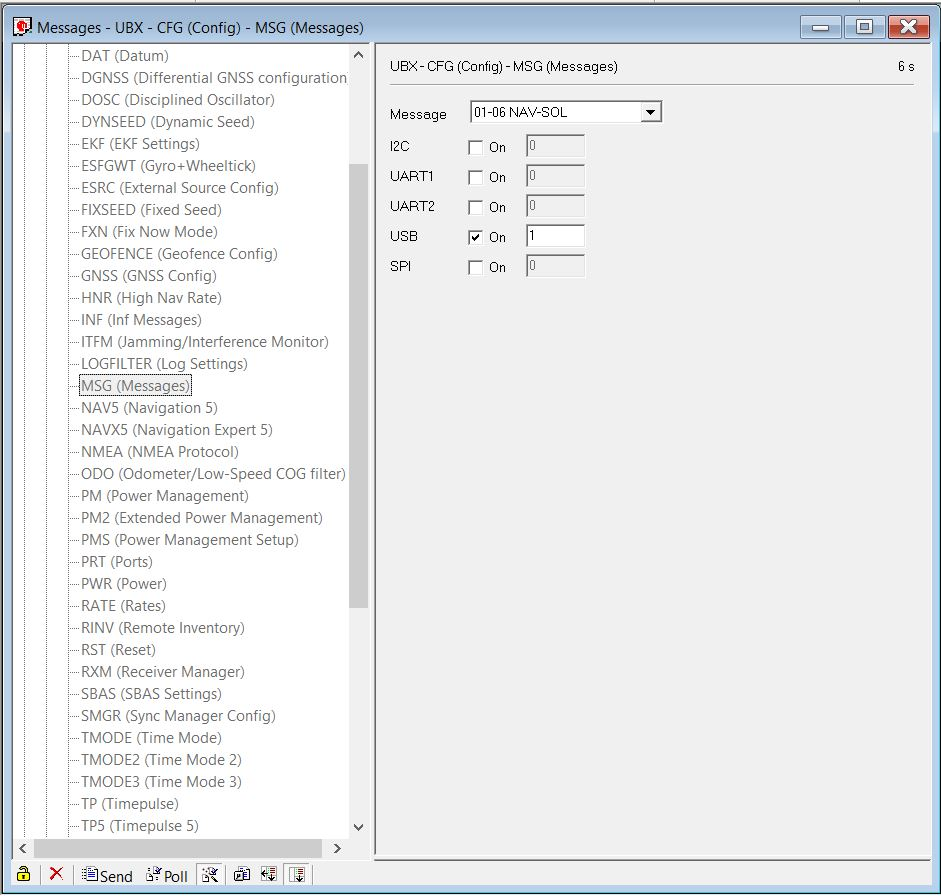
\includegraphics[width=0.5891036\linewidth]{Figures/Ublox/CapturaC_Base}}
\caption{Configuración de mensajes enviados mediante protocolo RTCM3.}
\label{fig:Mes_Base}
\end{figure}

En el cuadro de lista desplegable \textbf{Message}, seleccionar \textit{F5-05 RTCM3.1 1005}, \textit{F5-4D RTCM3.1 1077} y \textit{F5-05 RTCM3.1 1087}. Seleccionar en todos ellos únicamente el cuadro de \textit{UART1}, tal y como muestran las figuras~\ref{fig:1005_Base},~\ref{fig:1077_Base},~\ref{fig:1087_Base}.

\begin{figure}[H] % Example image
\center{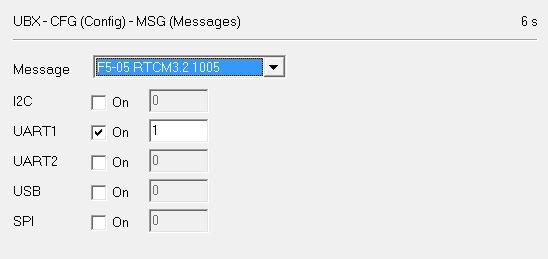
\includegraphics[width=0.5\linewidth]{Figures/Ublox/CapturaD_Base}}
\caption{Enviar mensaje 1005 mediante RTCM3.}
\label{fig:1005_Base}
\end{figure}

\begin{figure}[H] % Example image
\center{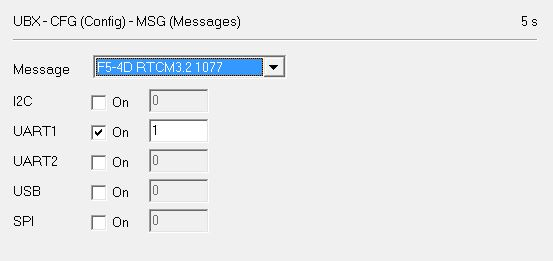
\includegraphics[width=0.5\linewidth]{Figures/Ublox/CapturaE_Base}}
\caption{Enviar mensaje 1077 mediante RTCM3.}
\label{fig:1077_Base}
\end{figure}

\begin{figure}[H] % Example image
\center{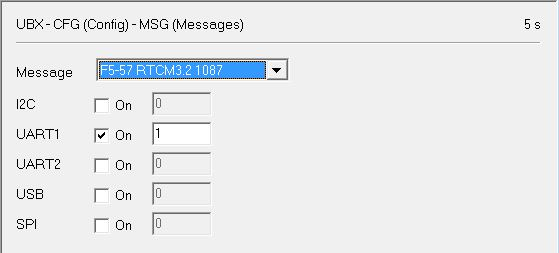
\includegraphics[width=0.5\linewidth]{Figures/Ublox/CapturaF_Base}}
\caption{Enviar mensaje 1087 mediante RTCM3.}
\label{fig:1087_Base}
\end{figure}

Dar clic al botón \textbf{Send} de la barra de herramientas inferior.\\

\subsection{Configurar la estación móvil}\label{SubChap:ConfMov}

Abrir el software U-Center y conectar el GPS que será designado a ser parte del Rover. Abrir la opción Messages View como en la subsección \ref{SubChap:ConfBase}.\\

Dar clic derecho a \textbf{NMEA}, de la lista de la parte izquierda, y seleccionar \textit{Deshabilitar} del menú contextual. Ahora dar clic derecho a \textbf{UBX} y seleccionar \textit{Habilitar}.\\

En la lista de la izquierda, seguir la ruta: \textbf{UBX - CFG (Config) - PRT (Ports)}. Saldrá una ventana como muestra la figura~\ref{fig:PRT_Rover}.

\begin{figure}[H] % Example image
\center{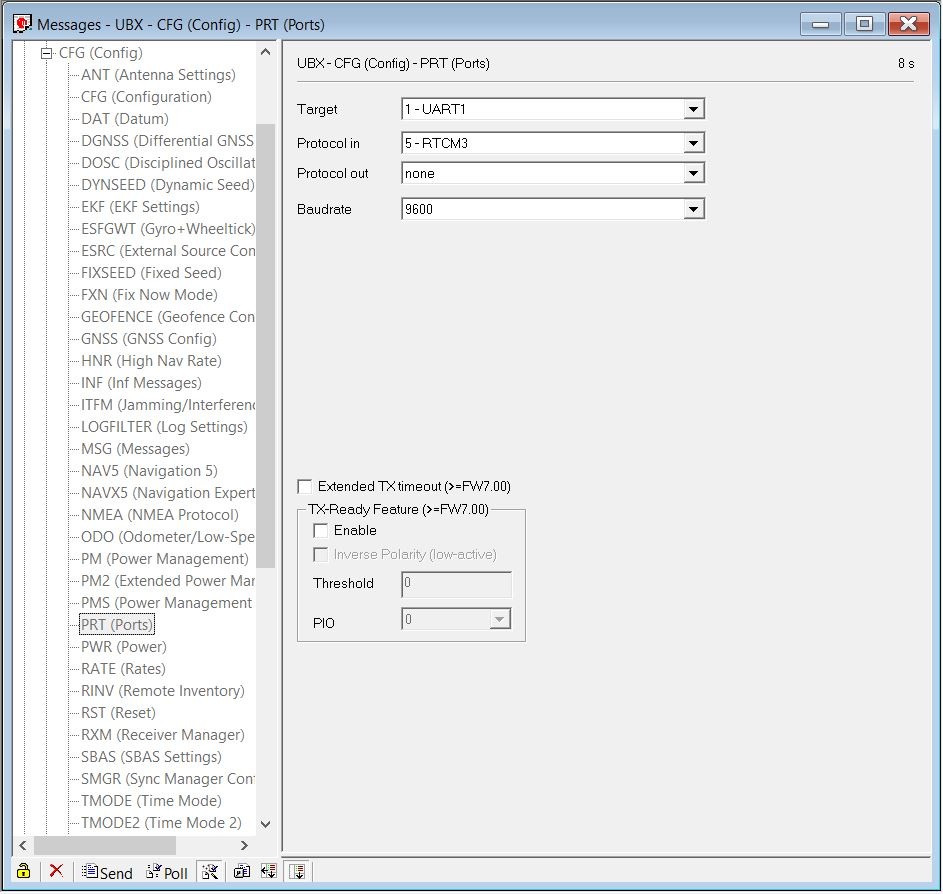
\includegraphics[width=0.75\linewidth]{Figures/Ublox/CapturaF_Rover}}
\caption{Configuración de comunicación del GPS rover.}
\label{fig:PRT_Rover}
\end{figure}

Se seleccionarán los siguientes parámetros:

\begin{itemize}
\item \textbf{Target}: \textit{1 - UART1}
\item \textbf{Protocol in}: \textit{5-RTCM3}
\item \textbf{Protocol out}: \textit{none}
\item \textbf{Baudrate}: \textit{9600}
\end{itemize}

Deshabilitar en caso de estar marcado \textit{Extended TX timeout(>=FW7.00)}.\\

Dar clic al botón \textbf{Send} de la barra de herramientas inferior.\\

Ahora, en la lista de la izquierda, seguir la ruta: \textbf{UBX - CFG (Config) - NAV5 (Navigation 5)} y se abrirá una ventana como la de la figura~\ref{fig:Nav_Rover}.

\begin{figure}[H] % Example image
\center{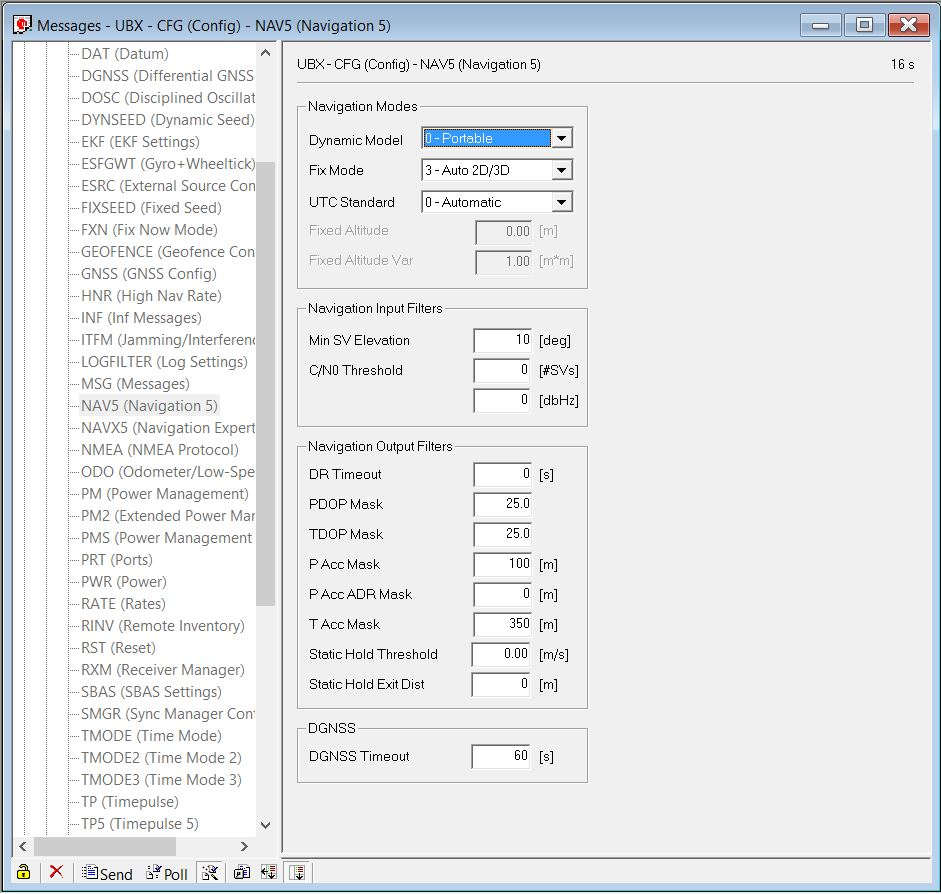
\includegraphics[width=0.75\linewidth]{Figures/Ublox/CapturaF_Rover2}}
\caption{Configuración de datos de navegación.}
\label{fig:Nav_Rover}
\end{figure}

Ingresar los siguientes parámetros:\\

En el área de \textit{Navigation Modes}
\begin{itemize}
\item \textbf{Dynamic Model}: \textit{0-Portable}
\item \textbf{Fix Mode}: \textit{3-Auto 2D/3D}
\item \textbf{UTC Standard}: \textit{0-Automatic}
\end{itemize}

El resto de parámetros dejarlos por default\footnotemark. \\

\footnotetext{Los parámetros por default se muestran en la figura~\ref{fig:Nav_Rover}.}

Dar clic al botón \textbf{Send} de la barra de herramientas inferior.\\

Lo único restante es guardar los datos de configuración en la memoria del GPS. Visitar en la lista de la izquierda la ruta: \textbf{UBX - CFG (Config - CFG (Configuration))}. Se abrirá una ventana como la de la figura~\ref{fig:SavAll}.

\begin{figure}[H] % Example image
\center{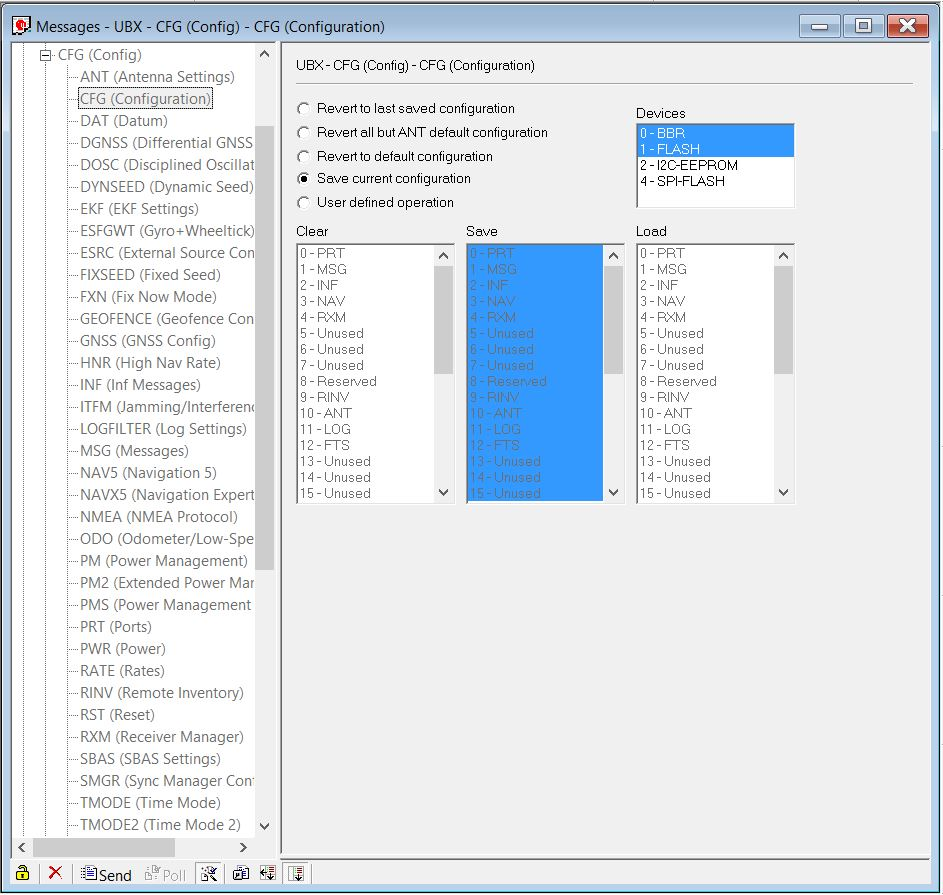
\includegraphics[width=0.75\linewidth]{Figures/Ublox/CapturaF_SaveAll}}
\caption{Guardado de la configuración.}
\label{fig:SavAll}
\end{figure}

Pulsar por última vez el botón \textbf{Send} de la barra de herramientas inferior. 

\section{Conclusión}

Tras seguir los pasos descritos en esta guía, los GPS Ublox C94-M8P se encuentran listos para ser conectados en sus respectivas estaciones para desempeñar su función. El designado a estar en la estación base enviará datos a su GPS par en el rover para que este último pueda depurar su posición, de acuerdo al fundamento de Real-Time Kinematics.

%\end{document}